\documentclass[a4paper, 11pt, final, garamond]{book}
\usepackage{cours-preambule}
\usepackage{pdfpages}

\raggedbottom

\makeatletter
\renewcommand{\@chapapp}{Travaux pratiques -- TP}
\makeatother

\let\SavedIndent\indent
\protected\def\indent{%
  \begingroup
    \parindent=\the\parindent
    \SavedIndent
  \endgroup
}
\setlength{\parindent}{0pt}

\begin{document}
\setcounter{chapter}{13}

\chapter{\'Etude d'un filtre actif du second ordre}

\section{Objectifs}

\begin{itemize}
    \item Être attentif-ve aux problèmes liés aux masses des appareils de
        mesure. 
    \item Apprécier rapidement le comportement en fréquence d'un filtre par
        balayage rapide avant de faire les mesures. 
    \item Effectuer les mesures permettant de tracer le diagramme de Bode en
        amplitude d'un filtre.
    \item Utiliser un multimètre en mode dBmètre.
    \item Apprendre à tracer un diagramme de Bode sur papier
        semi-logarithmique~: fréquence de coupure à $-\SI{3}{dB}$, bande
        passante, nature et ordre du filtre. 
\end{itemize}


\section{Méthode pour mesurer un gain en dB (rappel)}

Le gain se mesure grâce à un multimètre en fonction Volt alternatif (symbole
V$\sim$) puis dBmètre (bouton dB) pour activer la fonction dBmètre. Brancher le
multimètre sur l'entrée $e(t)$ du montage, appuyer sur «~rel~» une ou deux fois
jusqu'à ce que le multimètre affiche 0. On indique alors au multimètre que c'est
cette tension $e(t)$ qui sert de référence. Brancher ensuite le multimètre sur
la sortie $s(t)$. Il affiche directement le gain en dB.

\begin{brapp}{\includehand{-90}{0.8cm}}
    \centering
    \textbf{ATTENTION~: Il faut refaire le zéro relatif pour chaque fréquence.}
\end{brapp}

\section{Analyser}

\begin{minipage}{0.45\linewidth}

    Le filtre de \textsc{Rauch} est un filtre actif, c'est-à-dire qu'il est
    alimenté électriquement par un générateur extérieur pour fonctionner. Il
    repose sur l'utilisation de 5 dipôles passifs et d'un amplificateur
    opérationnel (AO). Ces derniers ne sont pas au programme de première année.
    Il n'est donc pas possible pour vous de déterminer la fonction de transfert
    associée à ce filtre. Vous pouvez donc voir le filtre comme une boîte noire
    qui réalise la fonction de transfert suivante~: 
    \[
        \boxed{
            \Hu(\jj \w) = \frac{\su}{\eu} = \frac{H_0}{1+\jj Q
            \left(\dfrac{\w}{\w_0}-\dfrac{\w_0}{\w}\right)}
        }
    \]
\end{minipage}
\hfill
\begin{minipage}{0.45\linewidth}
    \begin{center}
        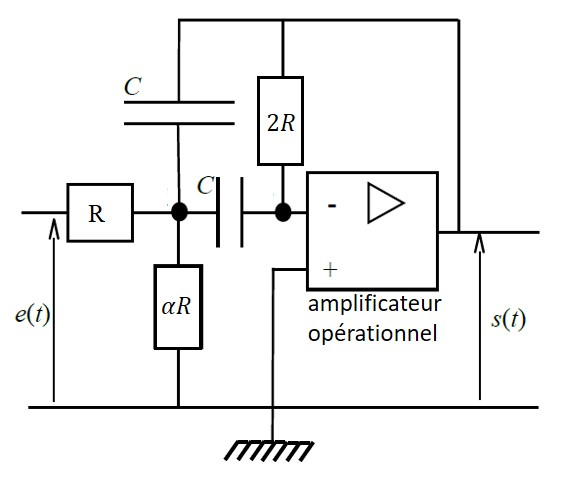
\includegraphics[width=\linewidth]{rauch_montage}
    \end{center}
\end{minipage}

\leftcenters{Avec}{$\DS Q = \sqrt{\frac{\alpha+1}{2\alpha}}, \quad H_0 = -1 \qet
\w_0 = \sqrt{\frac{\alpha+1}{2\alpha}} \, \frac{1}{RC}$}

\medskip

Ainsi, bien que ce filtre soit nouveau par rapport à ce que vous avez étudié, sa
fonction de transfert est analogue à des cas étudiés en classe. Vous pouvez donc
étudier sa fonction de transfert. Pour ce faire~: 
\begin{enumerate}[label=\sqenumi]
    \item Déterminer les équations des asymptotes BF et HF du Bode en gain. En
        déduire la nature de ce filtre.
    \item Exprimer la pulsation de résonance $\w_{r}$ en fonction de $\w_0$ et
        $Q$. Exprimer la largeur de la bande passante de ce filtre en fonction
        de $\w_0$ et $Q$, puis de $R$ et $C$.
    \item A quelle condition sur $\alpha$ ce filtre peut-il être efficace pour
        sélectionner individuellement les fréquences constituant le signal
        d'entrée~? On supposera, afin de fixer les idées, un signal d'entrée
        périodique (non sinusoïdal) de pulsation fondamentale $\w_{f}$ dont on
        souhaite sélectionner l'harmonique de rang 3 (pulsation $3\w_{f}$). 
    \item On prend $RC=\SI{1.0e-4}{s}$. Pour $\alpha= \num{e-2}$ puis $\alpha=1$,
        préciser les coordonnées des points d'intersection des asymptotes BF et
        HF $(f_{I}~;~G_{{\dB}, I})$. 
\end{enumerate}

\section{Réaliser}

On étudie ce montage pour deux valeurs de $\alpha$. On prendra successivement
$\alpha=\num{e-2}$ puis $\alpha=1$.

Le filtre schématisé ci-dessus est une «~boite noire~» dans laquelle on trouve
un amplificateur opérationnel. Pour s'en servir, il faut au préalable polariser
l'amplificateur opérationnel, c'est-à-dire~:

\begin{instruc}{Manipulation amplificateur}
    Connecter la borne \SI{+15}{V} du boitier à la sortie \SI{+15}{V} d'un
    générateur de tension continue, la borne \SI{-15}{V} du boitier à la sortie
    \SI{-15}{V} du générateur et le point milieu du boitier à la masse du
    générateur.
\end{instruc}

\begin{bror}{\includehand{-90}{0.8cm}}
    \centering\bfseries
    À la fin de la séance, on coupe le signal du GBF avant les alimentations de
    l'amplificateur opérationnel qui doivent être coupées en dernier.
\end{bror}

Réalisez ensuite le montage en prenant $C=\SI{1}{nF}$ (cavalier prêt à être
connecté sur la boite) et $\alpha R$ avec une boite de résistances variables.
\bigbreak

\begin{enumerate}[resume, label=\sqenumi]
    \item La «~boite noire~» a été fabriquée avec $R= \SI{100}{k\Omega}$.
        Déterminer la valeur à donner à $\alpha R$ pour $\alpha=\num{e-2}$. 
\end{enumerate}

\bigbreak
On alimente le filtre avec un GBF en tension sinusoïdale et on souhaite
visualiser simultanément $e(t)$ sur la voie 1 et $s(t)$ sur la voie 2 de
l'oscilloscpe. On utilisera le voltmètre pour mesurer le gain en dB. \bigbreak

\begin{enumerate}[label=\sqenumi, resume]
    \item \underline{Étude rapide}~: Faire varier la fréquence du signal
        d'entrée et vérifier rapidement que le filtre fonctionne correctement.
        En particulier, vous déterminerez la fréquence de résonance.
    \item \underline{Mesures pour le tracé du diagramme de Bode}~: Prendre comme
        amplitude du signal d'entrée $E_{m} \approx \SI{2}{V}$ puis, pour chaque
        fréquence entre $\SI{100}{Hz}$ et $\SI{80}{kHz}$, mesurer le gain en dB
        grâce au voltmètre (en mode dB-mètre, comme la semaine précédente) et
        affiner les mesures autour de la fréquence de résonance. L'échelle
        fréquentielle étant logarithmique, vous espacerez vos mesures de manière
        logarithmique également. Faire un tableau \textit{numérique} avec
        l'outil de votre choix (LatisPro recommandé, calculatrice recommandée)
        et imprimez ou réécrire les valeurs sur votre copie.
    \item Recommencer les deux mêmes études pour $\alpha=1$.
\end{enumerate}

\section{Valider}

\begin{enumerate}[label=\sqenumi, resume]
    \item Tracer, pour chacune des deux valeurs de $\alpha$, les diagrammes de
        Bode en gain expérimentaux sur papier semi-log en mettant la fréquence
        en abscisse. Ajouter sur ces deux diagrammes, les asymptotes obtenues
        grâce à l'étude théorique de l'analyse.
\end{enumerate}

\section{Conclure}

\begin{enumerate}[label=\sqenumi, resume]
    \item Quelle différence essentielle constate-t-on entre ces deux filtres~?
        Comment faire varier la capacité $C$ afin de faire varier $Q$ sans faire
        varier $\w_0$~? 
\end{enumerate}

\newpage

\thispagestyle{empty}
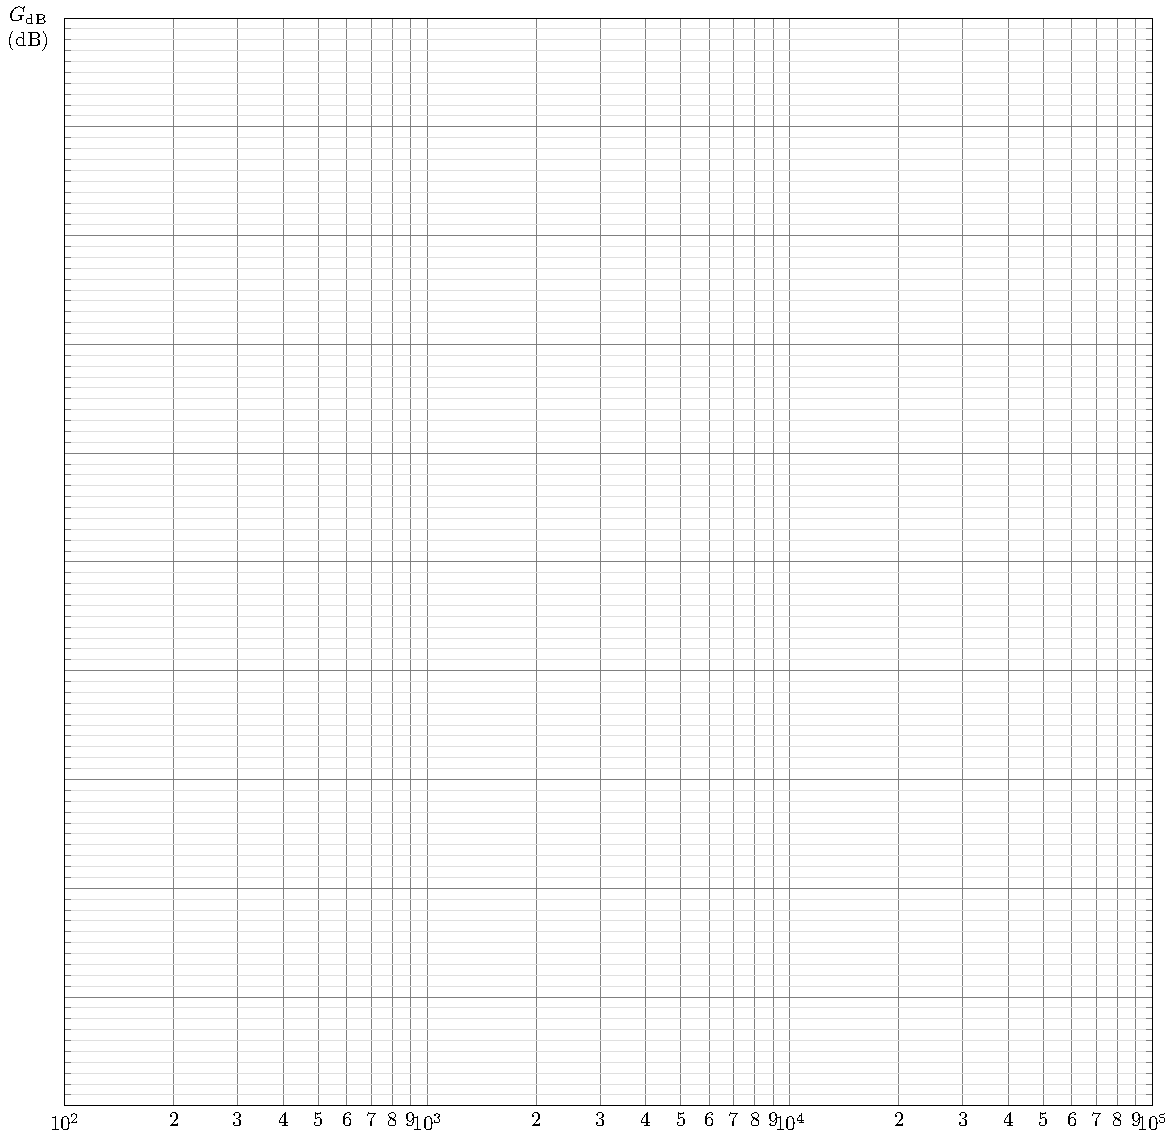
\includepdf{semilog}

\newpage

\thispagestyle{empty}
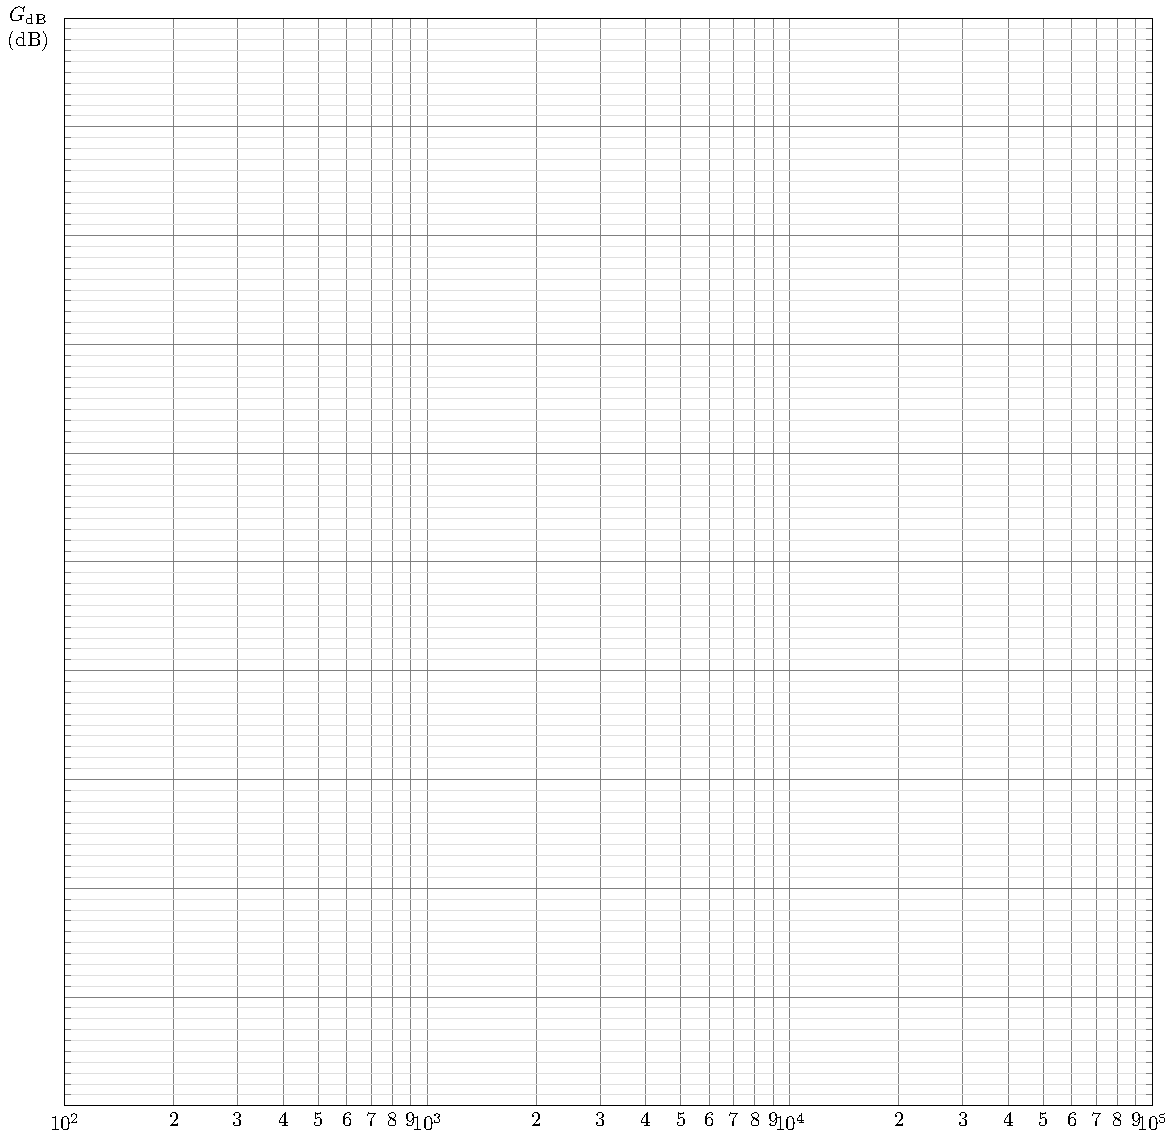
\includepdf{semilog}

\end{document}
